The $_{s}\mathcal{P}lot$ technique is a powerful tool that allows for the separation of different contributions in a dataset, 
typically signal and background. This technique relies on the modelling of a discriminating variable, where the distributions of each 
of the components are known, then a statistical reweighting of the data is performed. This reweighting applies $_{s}Weights$,
which reweights the data into 'signal-like\rq and 'background-like\rq data sets. The $_{s}\mathcal{P}lot$ technique is particularly useful 
when the signal and background distributions are not easily separable, or the distibutions of the components are not easily described.   
In our analysis, we employ a continuum reduction selection to effectively remove continatoric background contributions and enhance
the accuracy of our $_{s}\mathcal{P}lot$ fit. Furthermore, we use the "$J/\psi$-constrained" B mass as the distriminating variable, as 
this provides a cleaner B-mass peak, and so reduces contamination of the 'signal-like\rq distributions 

% Effect of application of CRS on constrained mass
\begin{figure}
    \centering
    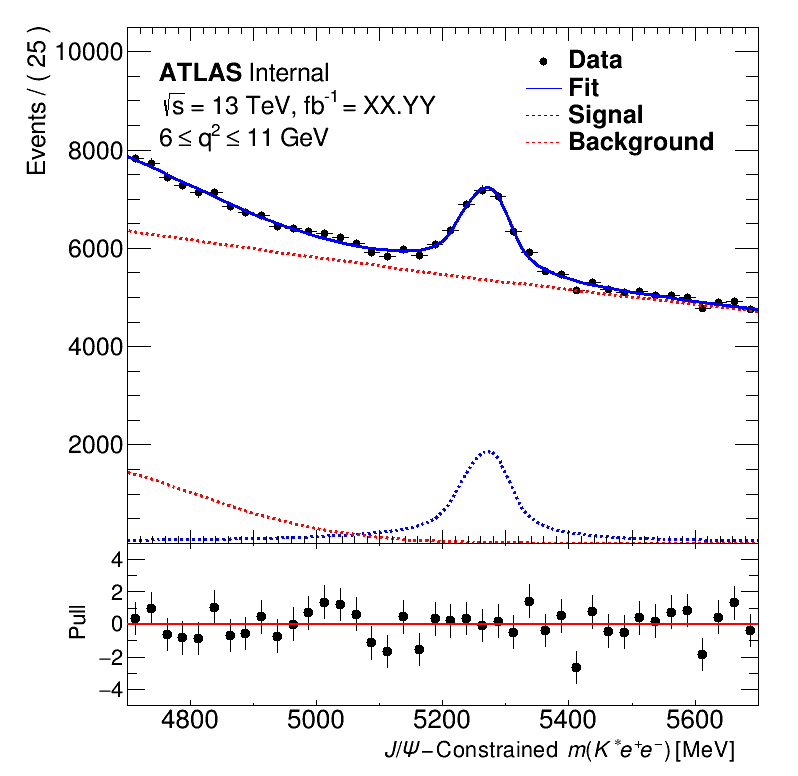
\includegraphics[width=0.45\textwidth]{figures/B_const_mass_CRS_before_eefit.png}
    \caption{Before the application of CRS on constrained mass.}
    \hfill
    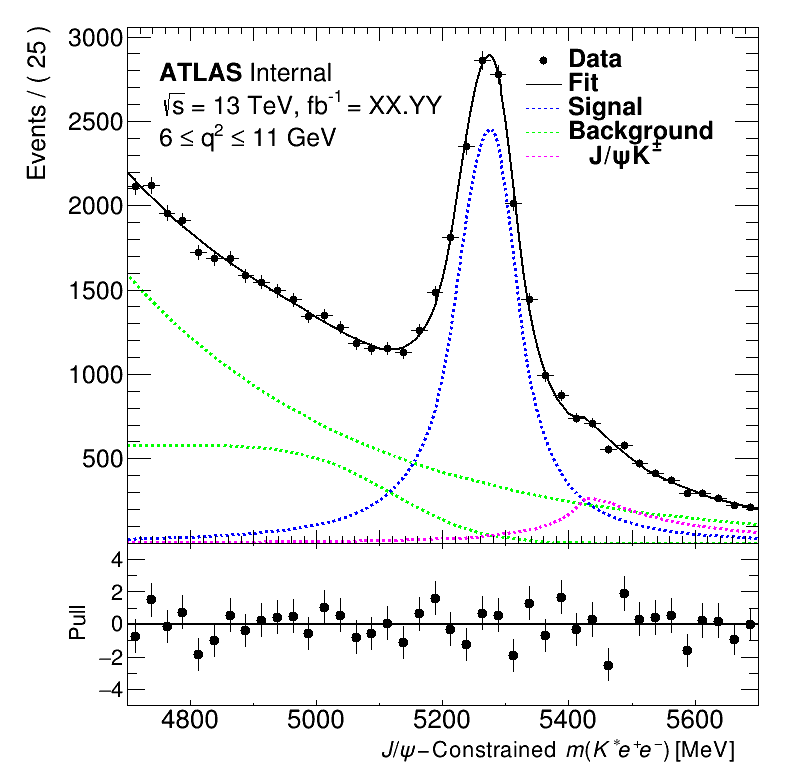
\includegraphics[width=0.45\textwidth]{figures/B_const_mass_CRS_after_eefit.png}
    \caption{After the application of CRS on constrained mass.}
    \label{fig:crs_effect_after}
\end{figure}

% MC fits to the signal and misreconstructed B+ mass distributions
\begin{figure}
    \centering
    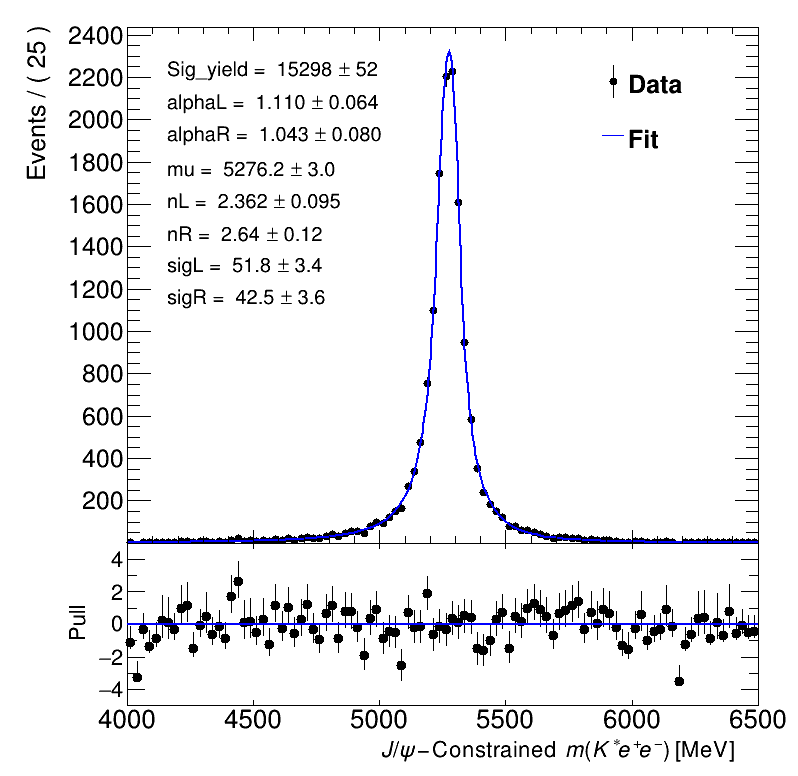
\includegraphics[width=0.45\textwidth]{figures/MC_B_const_mass_fit_signal.png}
    \caption{MC fit to the signal mass distribution.}
    \hfill
    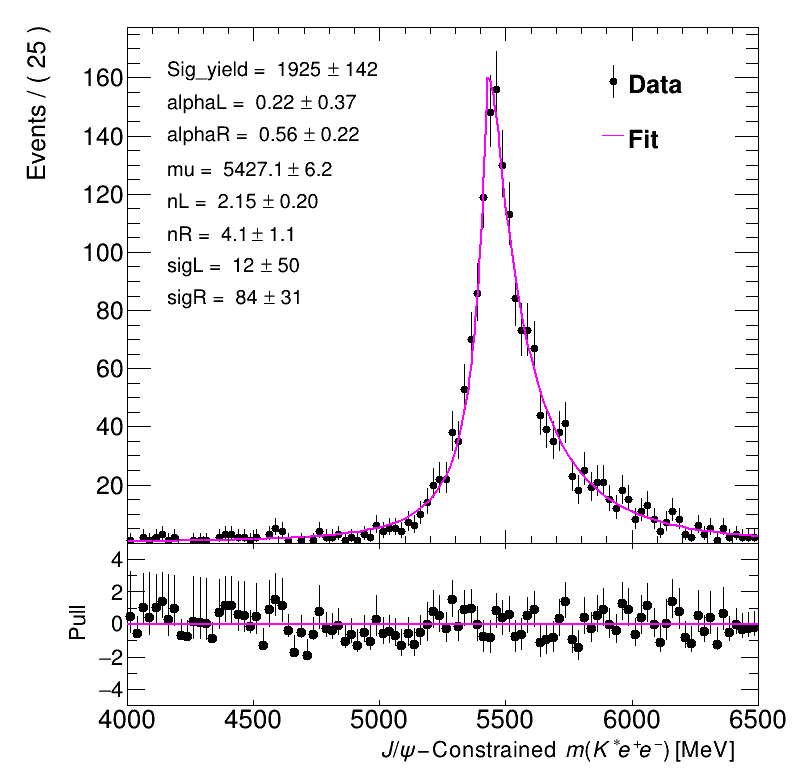
\includegraphics[width=0.45\textwidth]{figures/MC_B_const_mass_bplus.png}
    \caption{MC fit to the misreconstructed B+ mass distribution.}
    \label{fig:mc_fit_bplus}
\end{figure}

% Shape comparison between SS and OS backgrounds, fit to OS with fixed
\begin{figure}
    \centering
    \centering
    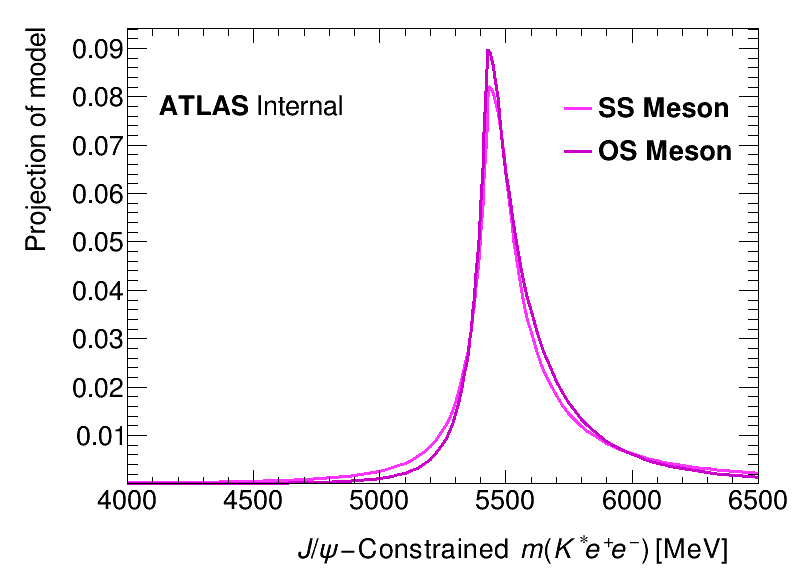
\includegraphics[width=0.3\textwidth]{figures/MC_B_const_mass_fit_OSvsSS.png}
    \caption{Fit to OS with free params.}
    \hfill
    \centering
    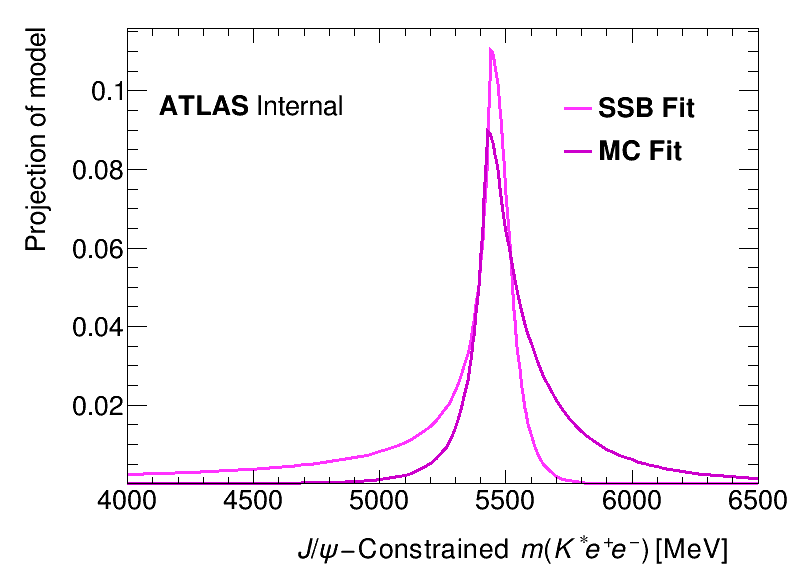
\includegraphics[width=0.3\textwidth]{figures/B_const_mass_shape_dataVsMC_OS.png}
    \caption{Fit to OS with fixed params.}
    \caption{Shape comparison between SS and OS backgrounds.}
    \label{fig:shape_comparison}
\end{figure}

\begin{figure}
    \centering
    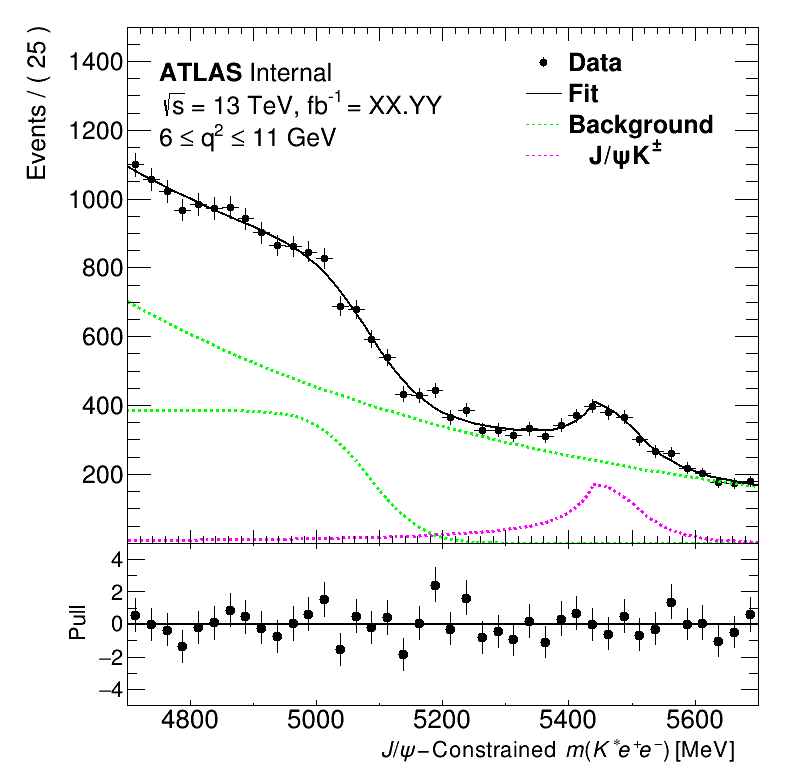
\includegraphics[width=0.8\textwidth]{figures/B_const_mass_CRS_high_OS_eefit_free.png}
    \caption{Fit to the OS high q2 data.}
    \label{fig:os_high_q2_fit}
\end{figure}

% Fit to the high q2 data with the B+ fix from the SSB - should be simultaneous? What about the backgrounds? - Same problem in the lowq2 region
\begin{figure}
    \centering
    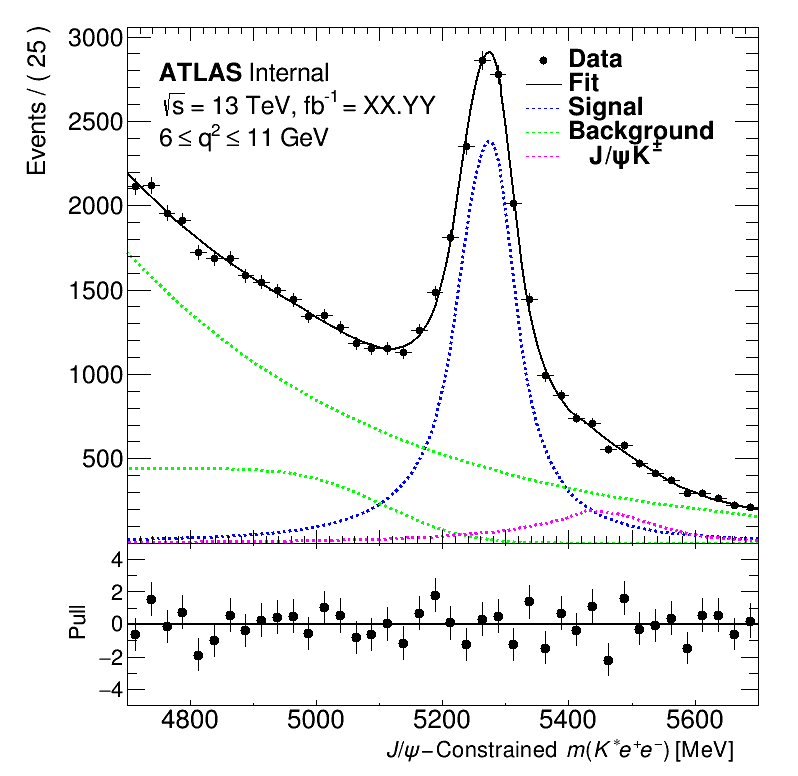
\includegraphics[width=0.8\textwidth]{figures/B_const_mass_CRS_high_q2_OSShapeFit_eefit.png}
    \caption{Fit to the high q2 data with the B+ fix from the SSB.}
    \label{fig:high_q2_fit_bplus}
\end{figure}

% Results of Splots
\begin{figure}
    \centering
    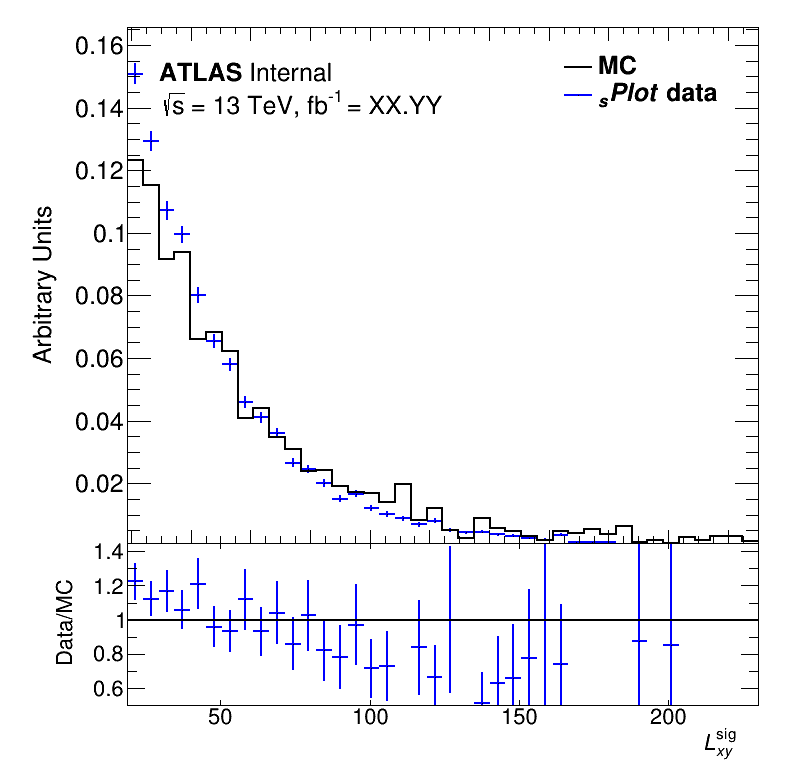
\includegraphics[width=0.25\textwidth]{figures/sPlot/splots_Lxysig.png}
    \hfill
    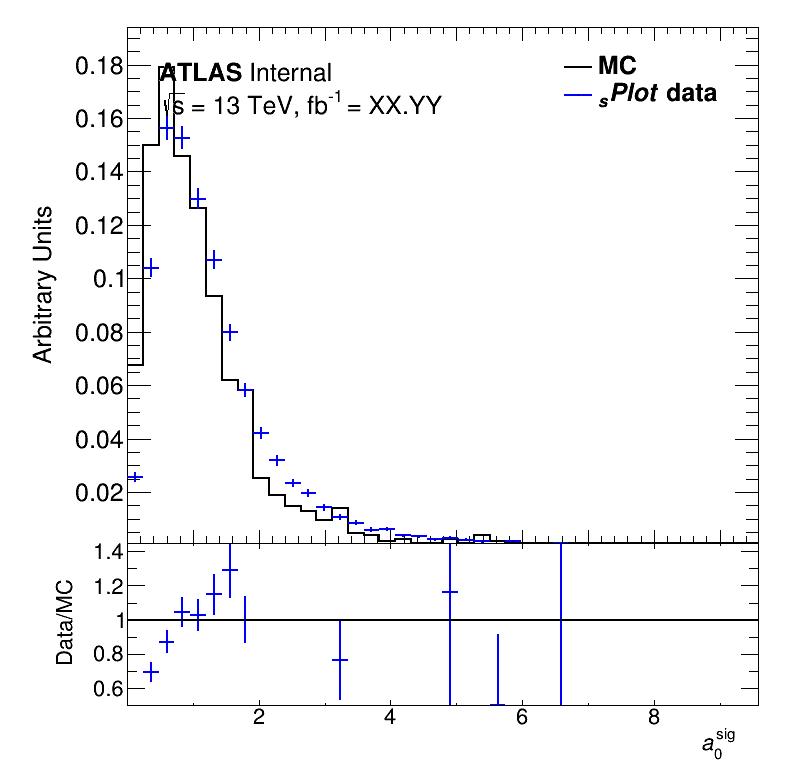
\includegraphics[width=0.25\textwidth]{figures/sPlot/splots_a0sig.png}
    \hfill
    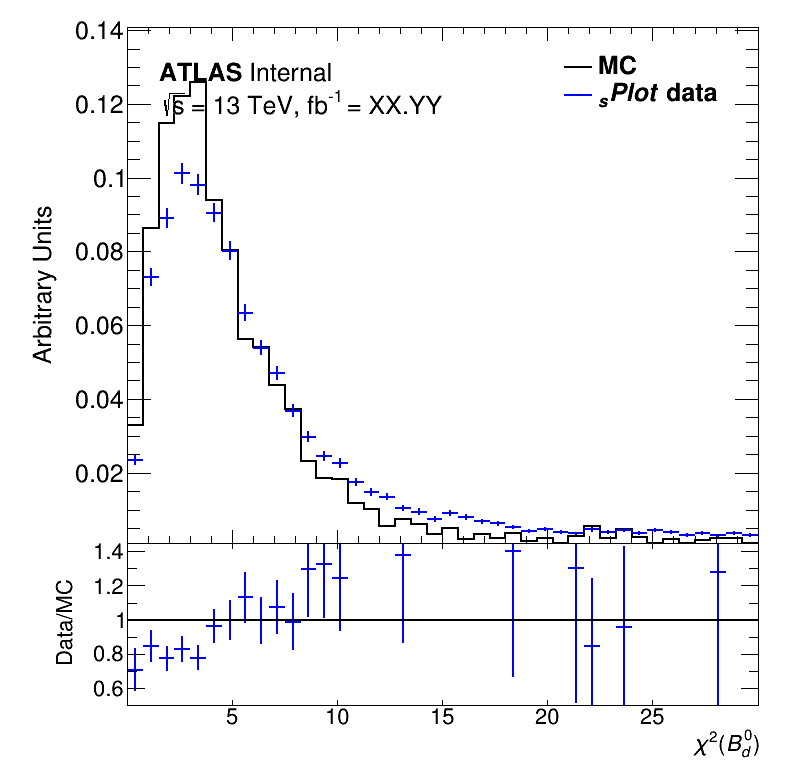
\includegraphics[width=0.25\textwidth]{figures/sPlot/splots_chi2.png}

    \vskip\baselineskip
    
    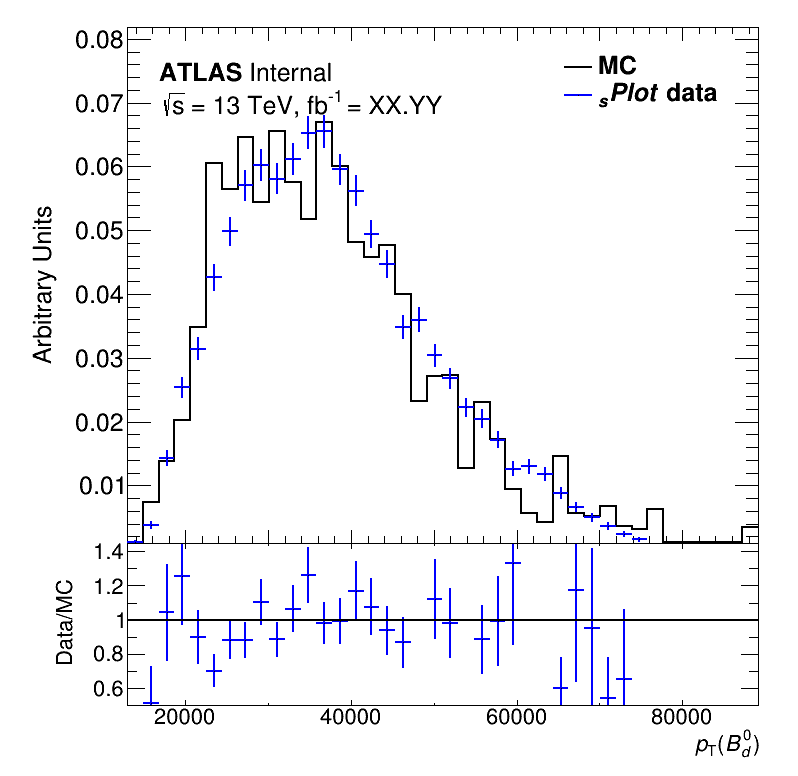
\includegraphics[width=0.25\textwidth]{figures/sPlot/splots_pTB.png}
    \hfill
    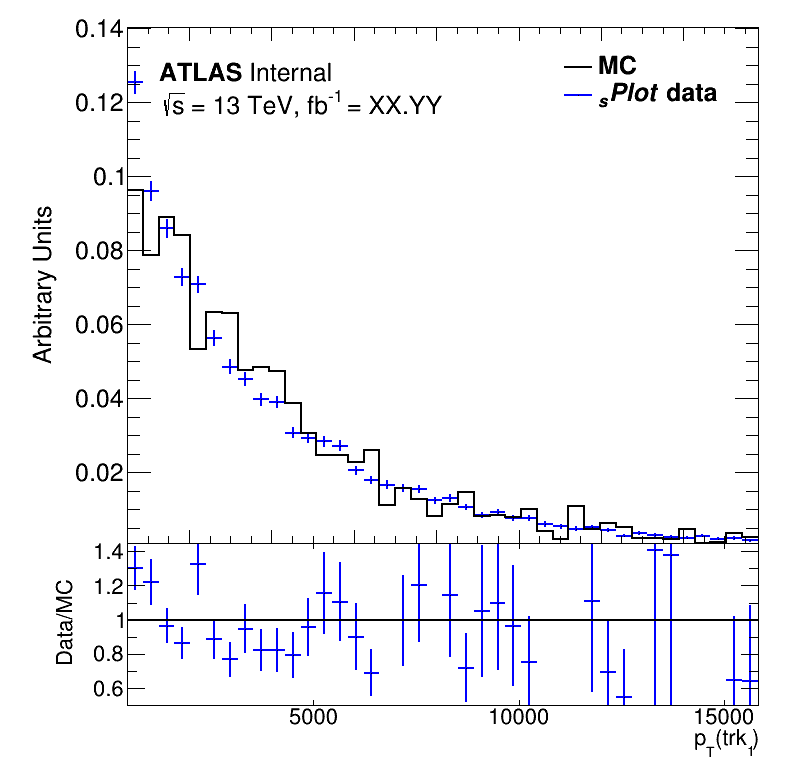
\includegraphics[width=0.25\textwidth]{figures/sPlot/splots_pTK.png}
    \hfill
    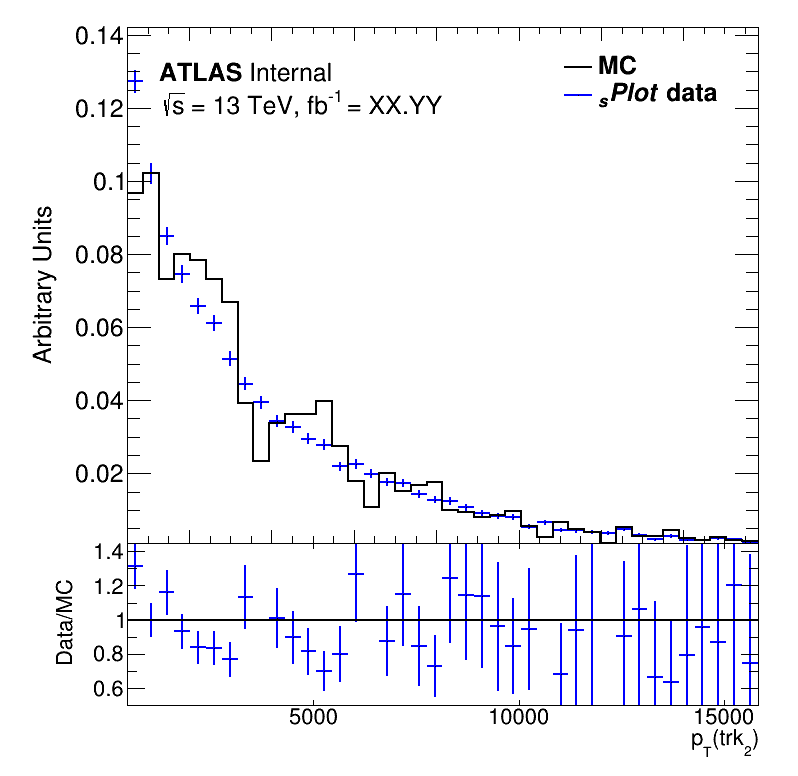
\includegraphics[width=0.25\textwidth]{figures/sPlot/splots_pTPi.png}    

    \caption{$_{s}\mathcal{P}lot$ results for the 6 most important input features to the GNN, where the trigger desicion and pile-up reweighting have been considered.}
    \label{fig:splots_results}
\end{figure}

    
